\subsubsection{Reserve a Taxi}
			To accompany this diagram, read the Scenario \hyperref[sec:TaxiReservationScenario]{S.10}.

				\begin{table}[htpb]
					\centering
					\label{tab:TaxiReservationTable}
					\begin{tabularx}{\textwidth}{lp{9cm}}
						\hline
						\hline
							\textbf{Subject}
						& 
							\textbf{Description}\\
						\hline
							Actors	       &  Customer, myTaxiService Web Application, myTaxiService Server\\
						\hline
							Preconditions  &  Customer must be on the homepage and is already logged in.\\
						\hline
							Execution      &  1.~Customer taps on the "Reserve a Taxi" button.\\
										   &  2.~myTaxiService Mobile Application shows the reservation page.\\
										   &  3.~Customer fills the reservation form.\\
										   &  4.~Customer submits the data by pressing "Reserve" button.\\
										   &  5.~myTaxiService Mobile Application calls the server function to reserve a taxi.\\
										   &  6.~myTaxiService Mobile Application shows a success notification.\\
						\hline
							Postconditions &  The Customer has reserved a taxi successfully.\\
						\hline
							Exceptions     &  1.~The Customer GPS is off.\\
							               &  2.~The Customer disconnects before reservation.\\
							               &  3.~The current time is less than two hour of the reservation time.\\
									
						\hline
						\hline
					\end{tabularx}
				\end{table}
				
				\begin{figure}[H]
					\centering
					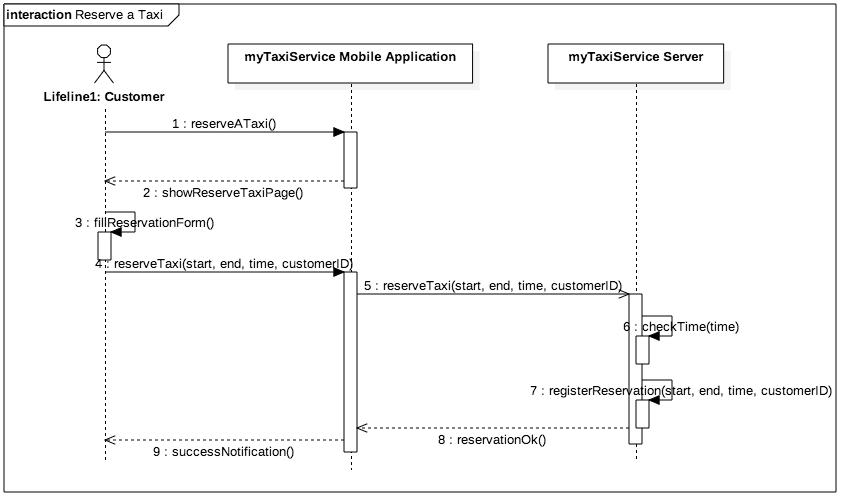
\includegraphics[width=\textwidth, scale=0.5]{IMG/InteractionDiagrams/TaxiReservation.png}
					\caption{Taxi Reservation Interaction Diagram}\label{sec:FigureTaxiReservation}
				\end{figure}